\documentclass[11pt]{article}
\setlength{\parindent}{0pt}


\usepackage{amssymb}
\usepackage{amsmath}
\usepackage{amsthm}
\usepackage{indentfirst}
\usepackage{graphicx}
\usepackage{graphicx}
\graphicspath{ {./images/} }


\begin{document}

\section*{MA 1024 Conference 6}

\vspace{\baselineskip}
\vspace{\baselineskip}

Ex 1) Double Integrals Over Rectangular Regions\\

Ex 2) Double Integrals Over General Regions \\

Ex 3) Double Integrals Over General Regions \\

Ex 4) Reversing the Order of Integration for Double Integrals\\

Ex 5) Finding Volume Under the Surface\\

Ex 6) Using Properties of Double Integrals\\

\newpage


\section*{Example 1 (Double Integrals Over Rectangles)}

Find $\int \int_{\; R} \, f(x,y) \, dA$, where $f(x,y) = (2x+3y)^{-2}$ and $R = [0,1] \times [1,2]$. \\

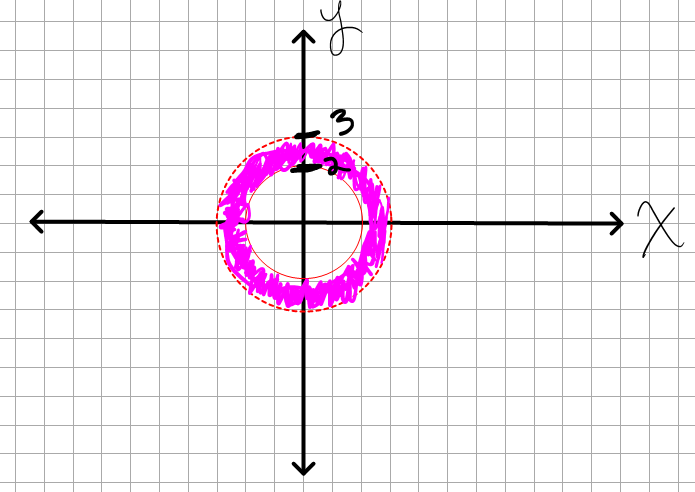
\includegraphics{Capture1.jpg}



\newpage

.

\newpage

\section*{Example 2 (Double Integrals Over General Regions)}

Find $\int \int_{\; R} \, f(x,y) \, dA$, where $f(x,y) = e^{\frac{x}{y}}$ and $R$ is the region given by the set $R = \{(x,y) \; | \; 1\leq y \leq 2, \; y\leq x \leq y^3\}$. \\

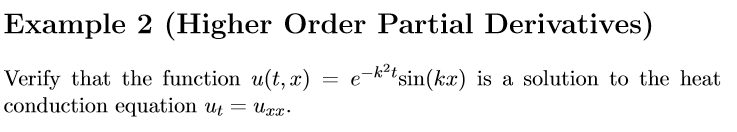
\includegraphics{Capture2.jpg}



\newpage

.

\newpage

\section*{Example 3 (Double Integrals Over General Regions)}

Find $\int \int_{\; R} xy$, where $R$ is the triangular region in the $xy$ plane with vertices $(0,0)$, $(6,0)$, and $(0,6)$. \\

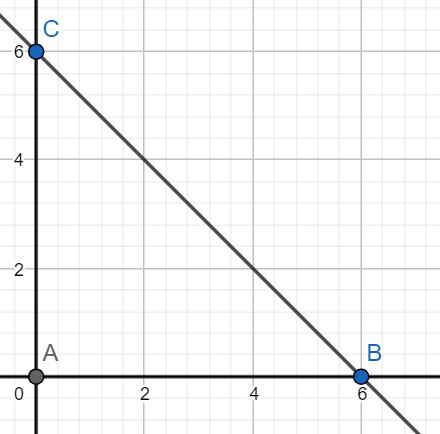
\includegraphics{Capture3.jpg}\\
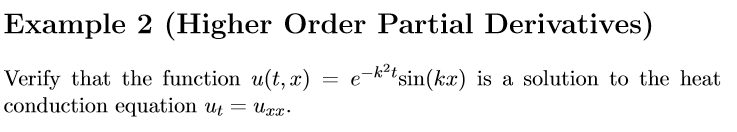
\includegraphics{Capture2.jpg}\\

(Problem repeated): Find $\int \int_{\; R} xy$, where $R$ is the triangular region in the $xy$ plane with vertices $(0,0)$, $(6,0)$, and $(0,6)$. \\

\newpage

.

\newpage

\section*{Example 4 (Reversing the Order of Integration)}

Evaluate the integral $I = \int_{0}^{8} \int_{\sqrt[3]{y}}^{2} \, \sqrt{x^4+1} \, dx \, dy$ by reversing the order of integration (using Fubini's Theorem). 




\newpage

.

\newpage

\section*{Example 5 (Double Integrals as Volume)}

Set up an integral to find the volume of the solid bounded by the planes $x=0$, $y=0$, $z=0$, and $x+y+z = 1$.



\newpage

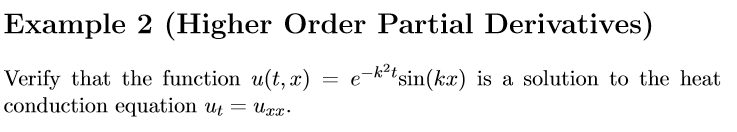
\includegraphics{Capture2.jpg}

\newpage


\section*{Example 6 (Properties of Double Integrals)}

Using the maxima of the function over the region $R$,
produce an upper estimate of the integral 

$$I = \int \int_{\; R} e^{x^2+y^2} \, dA$$

Where $R$ is the disk in the $xy$ plane with $x^2 + y^2 \leq 1$.

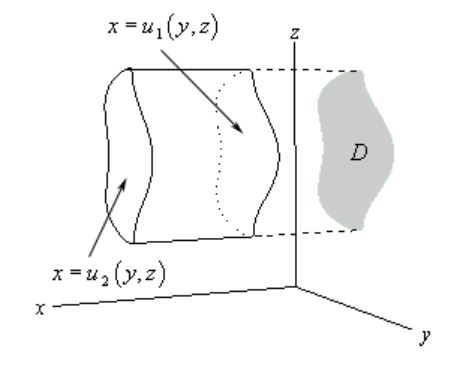
\includegraphics[scale = 0.85]{Capture4.jpg}\\

\includegraphics{Capture5.jpg}

\newpage

.

\newpage




\end{document}